% !TEX root = ../Thesis.tex

%requirements plusminus 2 pagina's
\section{Objectives (D)}
\label{sec:objectives}
In this section we give an overview of the most important objectives of this graduation project.
The complete list of objectives as given in the beginning of the project is given in the project planning \citepr{plan}.

\subsection{Ampersand project}
In November 2003, the Business Rules Manifesto \cite{business-rules} was written, with the main purpose of declaring independence for business rules in the world of requirements.
The manifesto supports the vision of business rules as equivalent to requirements.
This is considered a radical change on how people see the world of business architecture.

In December 2010, Stef Joosten, Lex Wedemeijer and Gerard Michels published the paper `Rule Based Design', presenting the Ampersand approach.
The approach puts the rules in the center, using these rules to define the business processes.
Ampersand is named after the \& symbol with the desire of realizing results for both business and IT, in an efficient and effective way.

In 2011, the Ampersand compiler was created as an open source project.
Since then, the compiler has been improved and applied in both business and academic contexts.
The Ampersand end-users write business rules in a specific language (ADL), and compile that specification into functional specification, documentation and working software prototypes.
\dict{ADL}{Ampersand Design Language}%
These rules are based on agreements between the different stakeholders.

The theory behind Ampersand has been thoroughly studied, and is based on mathe\-matical concepts, e.g. relational algebra and Tarski's axioms.
Using this compiler, users write the requirements in ADL and generate all the system specification independent of the platform.
The main advantage is that the requirement's consistency and traceability are always correct (and even provable), from the lowest level up to the front-end.
The requirements are presented to stakeholders in natural language, guaranteeing that any business expert who knows the context can validate the requirements.
\autoref{fig:generation} depicts the artifacts generated by the Ampersand compiler.
%
\begin{figure}[htb]
	\centering
	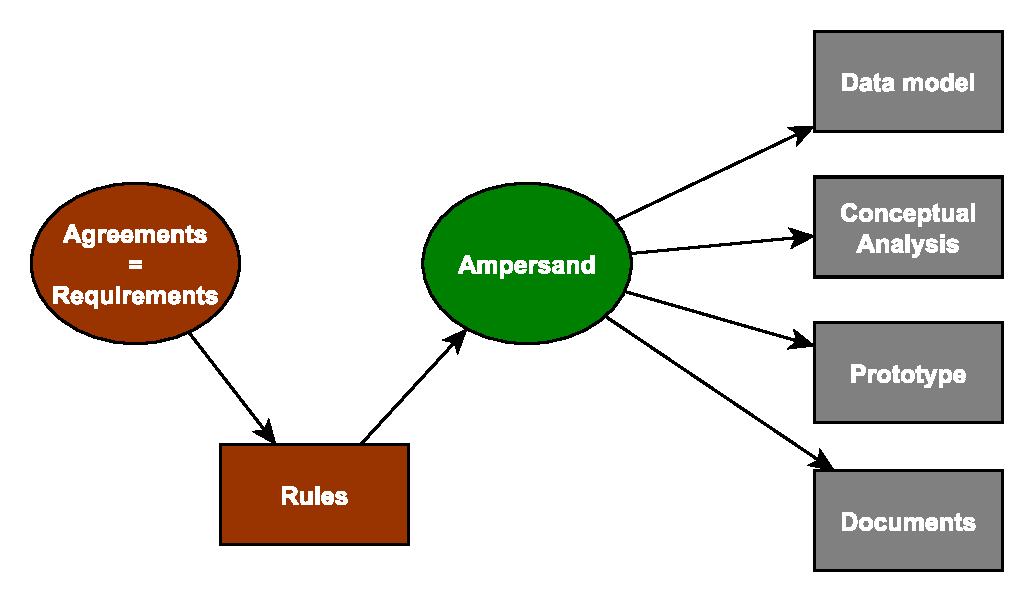
\includegraphics[width=0.7\textwidth]{Figures/Generation}
	\caption[Generated artifacts]{The Ampersand approach generates different artifacts based on the business rules (source: \cite{ampersand-approach})}
	\label{fig:generation}
\end{figure}
%

The Ampersand project is used in several environments, by different user groups.
In a research context, the Ampersand project is part of the research on the use of business rules for software design.
In an academic context, it is also used as the main tool in the course `Ontwerpen met bedrijfsregels' (code T18321) from the Open University of the Netherlands.
Finally, the compiler is used in business environments to design and develop real world business software.

\subsection{High-level architecture}
\label{subsec:architecture}
The compiler developed for the Ampersand research project runs in several steps, hence the Ampersand compiler is also divided in several subcomponents:
\dict{P-structure}{The parse-tree generated by the Ampersand parser, used as input for the type checker}%
\dict{A-structure}{The ADL code generated by the Ampersand type checker, used as input for the calculator component}%
\dict{ADL-structure}{See A-structure}%
\dict{F-structure}{The functional structure generated by the Ampersand calculator, used as input for the different output modules}%
\begin{description}
	\item[Parser:] This component receives the ADL code as input, and parses that code into a parse-tree (also known as P-structure).
	\item[Type checker:] The Ampersand type checker receives a P-structure as input and converts it into a relational algebra format, suitable for manipulation (also known as A-structure or ADL-structure).
		 The semantics of ampersand are expressed in terms of the A-structure.
	\item[Calc:] The Calc component receives an A-structure as input, and manipulates it according to the research rules, generating the functional structure (also known as F-structure).
		The F-structure contains all design artifacts needed to write a specification and generate the output.
	\item[Output components:] All design artifacts present in the F-structure are ready to be rendered.
		Several components use this data structure to generate the wished output.
		The output components currently implemented (and their output formats) are the following: 
		\begin{itemize}
			\item Atlas (HTML interface);
			\item Revert (Haskell source);
			\item Query (prototype generation);
			\item Documentation Generator (Pandoc structure).
		\end{itemize}
\end{description}

\subsection{Current situation}
The end-to-end process of the ampersand project, from compiling towards the generated artifacts, is correct, however there is a major improvement topic identified in the first step, the parsing of the input scripts.

One of the main complaints from users is the quality of the errors generated by the Ampersand parser making it hard for the end users to correct faulty ADL statements.
Since the beginning of the project, the parser subcomponent never received special attention, and it has not been analyzed for improvements.

In order to generate better, useful and to the point error messages, it is assumed that a complete refactoring of the parser will be necessary.
The main challenge is to choose the correct kind of architecture and libraries.

The main objective is to completely rebuild/refactor the Ampersand parser in order to give user-friendly error messages for the most common parsing errors.
Note that discovering which errors are the most common and what user-friendly messages consist of, is an important part of the assignment.
At the beginning of the project, no list of undesirable error messages is available.
It was up to us, as a part of the project, to judge which error messages were good enough and which were undesirable.

The first step was thus to investigate, document and understand the previous parser.

\subsection{Other objectives}
While designing and implementing the new Ampersand parser, the following objectives were also important:
\begin{description}
  \item [Libraries] because different implementation options are available, it was important to choose the most suitable Haskell parsing library.
  \item [Pretty-printing] is named in the project description.
  \item [Maintainability] had to be either maintained or improved; otherwise the parser wouldn't be taken into production.
  \item [Tests] had to be well-done, e.g. by using QuickCheck and other tools.
  \item [Tools] were important to support the software quality
  \item [Haskell]
  \item [Fixed syntax]
  \item [Fixed parse tree]
\end{description}

During the project, some additional requirements have been identified:
\begin{description}
  \item [Git/GitHub] the changed software had to be integrated into the GitHub Ampersand project.
    The development itself would happen in a separate branch of a separate fork, so that deliveries could be merged in a smooth way.
    This was an especially hard requirement for us, since we had no experience with Git.
  \item [Cabal] was used as a building platform.
  \item [EBNF] The syntax of the Ampersand grammar is specified in EBNF notation but was not up-to-date.
    Any changes to the syntax must be documented according with this notation.
    The notation can also be added as comment in the source code, in order to make clear that the complete grammar is implemented correctly.
\end{description}

On top of the project goals, the project members declare herewith to have the following personal objectives and commitments fulfilled by the end of this graduation project:
\begin{description}
	\item[Knowledge] Building up knowledge is the main reason why one starts a bachelor study.
		As such it is important to learn more about functional programming, Haskell, compilers, parsers, LaTeX, Ampersand, business rules and research in general.
	\item[University] Hopefully the final thesis will be of use for the university and other students.
	\item[Graduation] As this is a graduation project, it is natural to have the graduation as an important objective.
\end{description}
